\documentclass[sigconf]{acmart}

\usepackage{todonotes}
\usepackage{outlines}
\usepackage{amssymb}
\usepackage{listings}

% Copyright
%\setcopyright{none}
%\setcopyright{acmcopyright}
%\setcopyright{acmlicensed}
%\setcopyright{rightsretained}
%\setcopyright{usgov}
%\setcopyright{usgovmixed}
%\setcopyright{cagov}
%\setcopyright{cagovmixed}


% DOI
% \acmDOI{}

% ISBN
% \acmISBN{}

%Conference
\acmConference[GECCO '17]{the Genetic and Evolutionary Computation Conference 2017}{July 15--19, 2017}{Berlin, Germany}
\acmYear{2017}
\copyrightyear{2017}

% \acmPrice{15.00}


\begin{document}
\title{Analysis of Inductive Program Synthesis Techniques on General Program Synthesis Tasks}

\author{Edward Pantridge}
\affiliation{
	\institution{MassMutual Financial Group}
	\city{Amherst}
	\state{Massachusetts}
	\country{USA}
}
\email{epantridge@massmutal.com}

\author{Thomas Helmuth}
\affiliation{%
  \institution{Washington and Lee University}
  \city{Lexington} 
  \state{Virginia} 
}
\email{helmutht@wlu.edu}

\author{Nicholas Freitag McPhee}
\orcid{0000-0002-6495-2612}
\affiliation{%
  \institution{University of Minnesota, Morris}
  % \streetaddress{600 E. 4th Street}
  \city{Morris} 
  \state{Minnesota} 
  \postcode{56267}
}
\email{mcphee@morris.umn.edu}

\author{Lee Spector}
\affiliation{%
	\institution{Hampshire College}
	\city{Amherst}
	\state{Massachusetts}
	\country{USA}
}
\email{lspector@hampshire.edu}


\begin{abstract}
	A variety of inductive program synthesis (IPS) techniques have emerged from a spread of research fields in recent decades. However, these techniques have not been adequately compared on general program synthesis tasks. In this paper, several state-of-the-art methods of inductive program synthesis are compared across a set of problems involving the search for programs dealing with various data types, control structures and number of outputs. The problem set also spans tasks that are generally approached using languages at the level of machine code, assembly language, and higher level languages. Although there are many helpful metrics to consider when comparing these methods, this comparison is mainly focused on success rate. The systems investigated in this paper include: Flash Fill, Magic Haskeller, TerpreT, and Genetic Programming. After comparing the solution rates of these methods on the problem set, the results suggest that Genetic Programming and, to an extent, TerpreT are more capable of finding solutions than Flash Fill and Magic Haskeller.
\todo[inline]{Keywords}
\end{abstract}

%
% The code below should be generated by the tool at
% http://dl.acm.org/ccs.cfm
%
\begin{CCSXML}
<ccs2012>
<concept>
<concept_id>10011007.10011074.10011092.10011782.10011813</concept_id>
<concept_desc>Software and its engineering~Genetic programming</concept_desc>
<concept_significance>500</concept_significance>
</concept>
<concept>
<concept_id>10003752.10003809.10003716.10011136.10011797.10011799</concept_id>
<concept_desc>Theory of computation~Evolutionary algorithms</concept_desc>
<concept_significance>300</concept_significance>
</concept>
</ccs2012>
\end{CCSXML}

\ccsdesc[500]{Software and its engineering~Genetic programming}
\ccsdesc[300]{Theory of computation~Evolutionary algorithms}

\keywords{ACM proceedings, \LaTeX, text tagging}


\maketitle

\section{Introduction}

Since the creation of Inductive Program Synthesis (IPS) in the 1970s\cite{Kitzelmann2009}, researchers have been striving to create systems capable of generating programs competitively with human intelligence. Modern IPS methods often trace their roots to the fields of machine learning, logic programming, evolutionary computation and others.

The similarities and differences of these methods have been discussed\cite{Kitzelmann2009}, but their performance is rarely compared on problem sets that could provide concrete insight into the capabilities and limitations of each method.

A demonstrative problem set has been compiled that assess an IPS method's ability to work within a range of levels of abstraction\cite{Gaunt2016}, manipulate a variety of data types, produce complex control structures and produce an arbitrary number of outputs of various forms\cite{Helmuth2015b}.

This investigation is exclusively considering a methods ability to find solutions. Other measures, such as runtime or hardware models, are not discussed. In order to asses if a method can find solutions to a problem, the problem must first be phrased, in its entirety, to the method. This is not always possible.

The conclusions drawn from this comparison will speak to the flexibility of each considered method, as well as each method's success rate.

\section{Current State of the Art}

\subsection{Flash Fill}

Flash Fill is a program synthesis technique found in Microsoft Excel \cite{Gulwani2011}. It was designed to help non-programmers perform repetitive tasks that would otherwise require them to write Excel macro programs. It specializes in tasks that require string manipulations. 

To test Flash Fills performance with our problem set, an Excel spreadsheet with one column per input and one column for output was created for each problem. Each spreadsheet included training data, which had both the input and output column populated, and unseen testing data, which left the output column cells empty.

Flash Fill is deterministic and analytic, thus it was only run once per problem on a single data set.

Excel does not include a native vector or list data structure, and it is not clear what the best way to phrase problems that require vectors to Flash Fill. A string representation of vectors was attempted for some problems, as well as putting each item from each vector in a separate cell. These approaches occasionally yielded results, but it is not clear what the optimal usage is.

It is not possible to pose tasks to Flash Fill that required multiple outputs. This includes problems that require printing values in addition to returning an output. Asking Flash Fill to generate each output value in separate cell was considered, but this would be two separate tasks and would not be comparable to other the other IPS methods.

Flash Fill does not support vector types. If a problem specifies an input value will be a vector of a fixed length, the problem can be posed with each element of the vector in its own cell. If the vectors length is not fixed, this cannot be done, because a tabular structure cannot be formed. If a problem requires a vector output, it cannot be posed to Flash Fill with elements in their own cell because generating each output value would be a separate IPS task.

Due to these shortcomings of Flash Fill, there are a number of problems in this comparison that Flash Fill was unable to attempt. This is discussed more in section 4.

\subsection{MagicHaskeller}

MagicHaskeller is a web based that synthesizes functions in the Haskell programming language based on example function calls and their desired output in the form of a predicate. To do this, MagicHaskeller generates a stream of functions that have the same signature as the example function calls. This includes: the same number of inputs, the same input types, the same number of outputs and the same output types.

Generated functions are tested against the input predicate, and a sample of passing functions are presented to the user. The user can then "Exemplify" the suggested solution functions to see how they would behave given a variety of other inputs. If the user cannot find a solution function, more function can be generated until the entire stream has been processed.

This process relies heavily on memoization. Being a web hosted service, all MagicHaskeller users share the same dynamic programming table, and the users cannot select which functions are included when searching.

\begin{figure}
\begin{verbatim}
((f [1, 2, 3] == [0, 1, 2]) && (f [-1, 1] == [-2, 0]))  
\end{verbatim}
\caption{An example predicate that can be supplied to MagicHaskeller. This particular predicate produces a solution to the Decrement problem.}
\label{fig:MHpred}
\end{figure}

Figure \ref{fig:MHpred} shows an example input predicate. Notice that multiple nested predicates can be supplied. The number of nested predicates that can be given to MagicHaskeller is very limited, and if too many predicates are given the system will produce memory errors. This is a consequence of MagicHaskeller being a web hosted service where resources are shared between all users. Due to this limitation, it was not possible to give MagicHaskeller the same training dataset as the other IPS methods. Although this weakens the presented results, it speaks to the usability and flexibility of the MagicHaskeller system.

MagicHaskeller supports the common primitive data types such as: integers, floats, strings and characters. Vectors and tuples are also supported, witch greatly expands the number of problems that were able to be posed to MagicHaskeller.

MagicHaskeller only allows for the synthesis of functions that produce a single output value. In order to pose question that require multiple outputs, MagicHaskeller was given predicates that specified a tuple as an output. For problems that specify that values should be printed in addition to the output value, it was considered sufficient if MagicHaskeller could synthesis a program that produced a single string containing all printed values (including whitespace and newline) as an element of its output tuple.

Due to MagicHaskeller being hosted on the web, it is difficult to embed MagicHaskeller in other systems.

\subsection{TerpreT}

TerpreT is a recently developed, probabilistic programming language that is designed for inductive program synthesis. Problems are specified in the TerpreT language, which is then translated into four different back-end inference algorithms: Forward Marginals Gradient Descent (FMGD), Integer Linear Programming (ILP), Satisfiability modulo theories (SMT) and SKETCH.

The TerpreT system attempts to solve IPS problems using these back-end algorithms and returns source code containing the successful parameters found by the successful back-end algorithm, if one is present.

Note that there is currently no publicly available implementation of TerpreT and thus only results on benchmark problems provided by the original authors could be obtained. It would be extremely valuable to compare TerpreT's performance on the rest of the problem set using in this paper once an implementation becomes available.

\subsection{Genetic Programming}

Soon after the rise of evolutionary computations, John R. Koza recognized that evolution could be used for more than optimizing a fixed structure of values. In the 1990s, Koza built upon genetic algorithms in such a way that produced executable programs. This technique, named Genetic Programming (GP), is considered inductive program synthesis because it uses input-output examples (refered to as test cases in the field of GP) to evolve a function. In fact, IPS was one of the origional motivations for creating the field of GP\cite{Koza1992}. 

Genetic Programming works by generating a initial population of random programs. Traditionally these programs are represented as trees where non-leaf nodes each denote a function. The children of each non-leaf node are used as the arguments to their parents. Leaf nodes denote terminal values that could be either a constant or input value. This initial population of random programs then follows the cycle in Figure \ref{fig:evo}  until a solution is found or the run is considered a failure.

\begin{figure}[t]
\centering
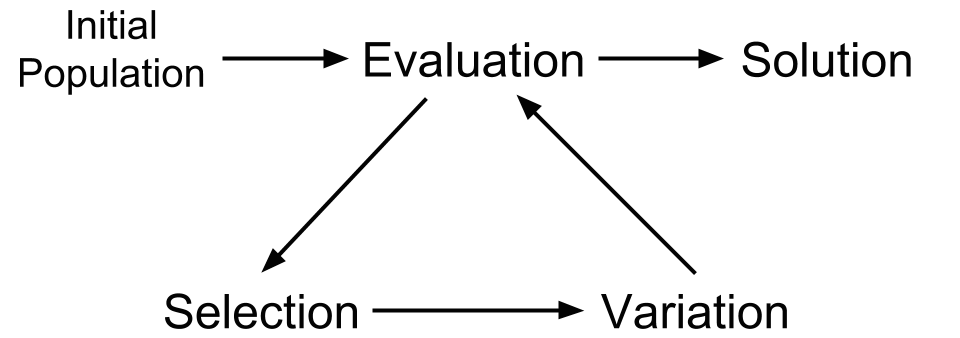
\includegraphics[width=0.25\textwidth]{res/EvolutionCycle}
\caption{Evolutionary Computation process.}
\label{fig:evo}
\end{figure}

\subsubsection{PushGP}

For this comparison, PushGP was selected as the Gennetic Programming method. PushGP evolves programs in a Turing complete, stack based language called Push. Push features separate stacks for each data type, including code. Push programs are lists of instructions and literals. Literals are values that get placed on the stack corrisponding to their type. Instructions are built-in functions that pop values off the stacks, modify them, and push them back on the appropriate stacks. Programs are run through an interpreter, which modifies the stacks. After all instructions and literals have been processed through the interpreter, the final state of the stacks is the output of the program \cite{Spector2002}.

\todo[inline]{Why PushGP for IPS?}

Implementations of PushGP systems are available in the Clojure programming language\footnote{https://github.com/lspector/Clojush}, as well as a new implementation in python\footnote{https://github.com/erp12/Pysh}.

\section{Problems}
\subsection{Basic Execution Models Problems}
The first set of problems were taken from \cite{Gaunt2016} and were intended to demonstrate TerpreT's ability to synthesis programs in a variety of execution models that span multiple levels of abstraction. These execution models are: Turing Machine, Boolean Circuits, Basic Block, and Assembly Language. 

As stated by \cite{Gaunt2016}, the problems in this set progress from more abstract execution models towards models which resemble assembly languages. This makes these problems demonstrative of how a system performs across a variety of low-level domains. 
 
The problems in this set are describes below:

\subsubsection{Invert}

Given a binary string (binary tape), invert all the bits.

\subsubsection{Prepend Zero}

Insert a $0$ in the first index of a binary string and shift all other bits to the right.

\subsubsection{Binary Decrement}

Given an input binary string equal to a positive decimal number, return a binary string equal to the input number decremented by one.

\subsubsection{2-bit Controlled Shift Register}

Given input bit ($r_1$, $r_2$, $r_3$), return the same bits, except swap the order of $r_2$ and $r_1$ if $r_1 == 1$.

\subsubsection{Full Adder}

Given a carry bit, $c_{in}$, and two argument bits, $a$ and $b$ , output a sum bit, $s$, and carry bit, $c_{out}$, such that  $s + 2c_{out} = c_{in} + a_1 + b_1$.

\subsubsection{2-bit Adder}

Given input bits $a_1$, $a_2$, $b_1$, and $b_2$, output $s_1$, $s_2$, and $c_{out}$ such that  $s_1 + 2s_2 + 4c_{out} = a_1 + b_1 + 2(a_2 + b_2)$.

\subsubsection{Access}

Given an input array, $V$, and a positive integer, $i$, return $V_i$. Assume $0 < i < |A|$.

\subsubsection{Decrement}

Given an input array, $V$ return a new array, $U$ such that $U_i = V_i - 1$.


\subsection{General Program Synthesis Benchmark Suite}
The second set of problems used in this comparison was proposed by \cite{Helmuth2015b} in order to provide the field of Genetic Programming with a set of non-trivial benchmark problems.

This problems set included problems that deal with multiple data types, including strings, numbers, boolean and vectors. There are also multiple problems in the set that require multiple output values, or printing certain values to the screen.

Given that the Basic Execution Models problem set is designed to test a systems ability to perform in low-level domains (binary circuits, assembly language, etc), the General Program Synthesis Benchmark Suite is an excellent addition, given that the problems' origins assume a much higher-level implementation (ie. java).

%\subsubsection{Number IO}
%\subsubsection{Small or Large}
%\subsubsection{For Loop Index}
%\subsubsection{Compare String Lengths}
%\subsubsection{Double Letters}
%\subsubsection{Collatz Numbers}
%\subsubsection{Replace Space with Newline}
%\subsubsection{String Differences}
%\subsubsection{Even Squares}
%\subsubsection{Wallis Pi}
%\subsubsection{String Lengths Backwards}
%\subsubsection{Last Index of Zero}
%\subsubsection{Vector Average}
%\subsubsection{Count Odds}
%\subsubsection{Mirror Image}
%\subsubsection{Super Anagrams}
%\subsubsection{Sum of Squares}
%\subsubsection{Vectors Summed}
%\subsubsection{X-Word Lines}
%\subsubsection{Pig Latin}
%\subsubsection{Negative To Zero}
%\subsubsection{Scrabble Score}
%\subsubsection{Word Stats}
%\subsubsection{Checksum}
%\subsubsection{Digits}
%\subsubsection{Grade}
%\subsubsection{Median}
%\subsubsection{Smallest}
%\subsubsection{Syllables}

\section{Results}

\todo[inline]{Which problems were not able to be posed to certain systems}
\todo[inline]{Which systems performed better on which problems}

\begin{figure}
\begin{tabular}{ r | c c c c }
	& TerpreT & Flash Fill & MH & PushGP \\
	\hline
	Invert & \checkmark & x & \checkmark & \checkmark \\
	Prepend Zero & \checkmark & \checkmark & \checkmark & \checkmark \\
	Binary Decrement & \checkmark & x & x & x \\
	2BCSR & \checkmark & x & x & \checkmark \\
	Full Adder & \checkmark & x & x & \checkmark \\
	2 Bit Adder & \checkmark & x & x & x \\
	Access & \checkmark & x & \checkmark & \checkmark \\
	Decrement & \checkmark & x & \checkmark & \checkmark \\
\end{tabular}
\caption{Results of all 4 systems on the Basic Execution Models problems from \cite{Gaunt2016}.  A check denotes the system could find a solution. An x denotes the problem was fully posed to the system, but a solution was not found. All problems were able to be fully posed to each system.}
\label{fig:results1}
\end{figure}

\begin{figure}
\begin{tabular}{ r | c c c c }
	& Flash Fill & MH & PushGP \\
	\hline
	Number IO & x & \checkmark & \checkmark  \\
	Small Or Large & x & x & \checkmark  \\
	For Loop Index &   & x & \checkmark  \\
	Compare String Lengths & ? & x & \checkmark  \\
	Double Letters & ? & x & \checkmark  \\
	Collatz Numbers & ? & x & x \\
	Replace Space with Newline &   & x & \checkmark  \\
	String Differences &   & x & x \\
	Even Squares &   & x & \checkmark  \\
	Wallis Pi & ? & x & x \\
	String Lengths Backwards &   & \checkmark  & \checkmark \\
	Last Index of Zero & ? & x & \checkmark  \\
	Vector Average & ? & \checkmark & \checkmark  \\
	Count Odds & ? & x & \checkmark  \\
	Mirror Image & ? & x & \checkmark  \\
	Super Anagrams & ? & x & \checkmark  \\
	Sum of Squares & ? & x & \checkmark  \\
	Vectors Summed & ? & \checkmark & \checkmark  \\
	X-Word Lines &   & x & \checkmark  \\
	Pig Latin & ? & x & \checkmark  \\
	Negative To Zero &   & \checkmark & \checkmark  \\
	Scrabble Score & ? & x & \checkmark  \\
	Word Stats &   & x & x \\
	Checksum & ? & x & x \\
	Digits &   & x & \checkmark  \\
	Grade & ? & x & \checkmark  \\
	Median & ? & x & \checkmark  \\
	Smallest & ? & \checkmark & \checkmark  \\
	Syllables & ? & x & \checkmark  \\
\end{tabular}
\caption{Results of all 3 systems on the Software Synthesis Benchmark Suite from \cite{Helmuth2015b}. A check denotes the system could find a solution. An x denotes the problem was fully posed to the system, but a solution was not found. No symbol denotes the problem could not be fully posed to the system.}
\label{fig:results2}
\end{figure}




\section{Conclusion}

\todo[inline]{Limitations of the comparisons.}
\todo[inline]{What does this mean for applications of IPS.}

\section{Things to mention somewhere}
\begin{itemize}
 \item Differences in runtime
 \item FashFill and MagicHaskeller come up with same thing every time. GP might not.
 \item Can you extract the solution program? Is it readable?
 \item We used boolean vectors as binary tape from TerpreT problems.
 \item We considered the Access problem and the List-k problem to be synonymous in most contexts.
\end{itemize}

\section{Acknowledgements}

This material is based upon work supported by the National Science Foundation under Grants No. 1617087, 1129139 and 1331283. Any opinions, findings, and conclusions or recommendations expressed in this publication are those of the authors and do not necessarily reflect the views of the National Science Foundation.

\bibliography{ss} 
\bibliographystyle{ACM-Reference-Format}

\end{document}

